\documentclass[aspectratio=169]{beamer}

\mode<presentation>
{
  \usetheme{default}
  \usecolortheme{default}
  \usefonttheme{default}
  \setbeamertemplate{navigation symbols}{}
  \setbeamertemplate{caption}[numbered]
  \setbeamertemplate{footline}[frame number]  % or "page number"
  \setbeamercolor{frametitle}{fg=white}
  \setbeamercolor{footline}{fg=black}
} 

\usepackage[english]{babel}
\usepackage[utf8x]{inputenc}
\usepackage{tikz}
\usepackage{courier}
\usepackage{array}
\usepackage{bold-extra}
\usepackage{minted}
\usepackage[thicklines]{cancel}

\xdefinecolor{dianablue}{rgb}{0.18,0.24,0.31}
\xdefinecolor{darkblue}{rgb}{0.1,0.1,0.7}
\xdefinecolor{darkgreen}{rgb}{0,0.5,0}
\xdefinecolor{darkgrey}{rgb}{0.35,0.35,0.35}
\xdefinecolor{darkorange}{rgb}{0.8,0.5,0}
\xdefinecolor{darkred}{rgb}{0.7,0,0}
\definecolor{darkgreen}{rgb}{0,0.6,0}
\definecolor{mauve}{rgb}{0.58,0,0.82}

\title[2017-10-13-lpc-testdrive]{New software for offline analysis}
\author{Jim Pivarski}
\institute{Princeton University -- DIANA}
\date{October 13, 2017}

\begin{document}

\logo{\pgfputat{\pgfxy(0.11, 7.4)}{\pgfbox[right,base]{\tikz{\filldraw[fill=dianablue, draw=none] (0 cm, 0 cm) rectangle (50 cm, 1 cm);}
\includegraphics[height=1 cm]{diana-hep-logo.png}}}}

\begin{frame}
  \titlepage
\end{frame}

% Uncomment these lines for an automatically generated outline.
%\begin{frame}{Outline}
%  \tableofcontents
%\end{frame}

%%%%%%%%%%%%%%%%%%%%%%%%%%%%%%%%%%%%%%%%%%%%%%%%%%%%%%%

%%%% START

%% \begin{frame}{Purpose of this talk}
%% \vspace{0.15 cm}
%% \begin{center}
%% \large To show you some of the software packages I've been developing \underline{so you can use them} and either get more productive or send me critical feedback.

%% \vspace{1 cm}
%% \uncover<2->{(I'm looking for beta testers.)}
%% \end{center}
%% \end{frame}

%% \begin{frame}{What is this software for, in the long run?}
%% \vspace{0.15 cm}
%% \large Ultimately, I and several others\footnote{Oliver Gutsche, Igor Mandrichenko (FNAL), Tanu Malik (DePaul CS), \mbox{Jean-Roch Vlimant (CalTech),\hspace{-1 cm}} Manos Karpathiotakis, Miguel Branco, Ioannis Alagiannis, Anastasia Ailamaki (EPFL/ATLAS)\ldots} want to develop a centralized service that will make plots more rapidly than you can with local skims.

%% \vspace{0.5 cm}
%% \uncover<2->{Think Google-for-HEP data. You submit a query and get a response on a short enough timescale to influence your next question.}

%% \vspace{0.5 cm}
%% \uncover<3->{We're still at the stage of testing various options, but meanwhile, I've been developing fast data access methods that you can use now, independently of any query system.}

%% \vspace{0.5 cm}
%% \uncover<4->{You can use it on your skims. (Same tools, different purpose.)}
%% \end{frame}

%% \begin{frame}{}
%% \begin{center}
%% \LARGE What I'll be showing today are various tools \\ for doing offline analysis faster.
%% \end{center}
%% \end{frame}

%% \begin{frame}{}
%% \vspace{1.2 cm}
%% \textcolor{darkblue}{Mental model of computing performance:} it isn't about speeding up your code, it's about {\it not slowing it down.} The mathematical function you want to compute has a fundamental speed set by the clock rate: everything else just gets in the way.

%% \begin{center}
%% 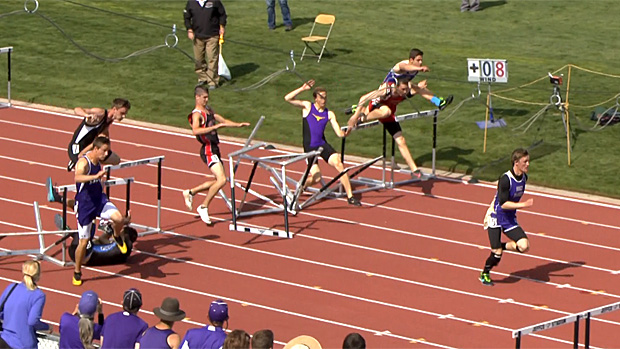
\includegraphics[width=0.7\linewidth]{hurdle9.jpg}
%% \end{center}
%% \end{frame}

%% \begin{frame}[fragile]{Experiment to try sometime}
%% \vspace{0.25 cm}
%% \begin{center}
%% \textcolor{darkorange}{\bf How long \underline{should} it take to compute an analysis function?}
%% \end{center}

%% \small
%% \begin{uncoverenv}<2->
%% \begin{minted}{python}
%% from time import *; from numpy import *; from math import *

%% pt1, pt2 = [random.normal(100, 10, int(1e6)) for i in 1, 2]
%% eta1, eta2 = [random.uniform(-5, 5, int(1e6)) for i in 1, 2]
%% phi1, phi2 = [random.uniform(-pi, pi, int(1e6)) for i in 1, 2]

%% start = time()
%% mass = sqrt(2*pt1*pt2*(cosh(eta1 - eta2) - cos(phi1 - phi2)))
%% end = time()

%% print(end - start)
%% \end{minted}
%% \end{uncoverenv}

%% \normalsize
%% \vspace{-0.75 cm}\hfill\begin{minipage}{0.35\linewidth}
%% \begin{uncoverenv}<3->
%% \begin{center}
%% \textcolor{darkblue}{$10^6$~events / 0.24 sec = 4.16~MHz}

%% \vspace{0.25 cm}
%% We need to get used to numbers like this.
%% \end{center}
%% \end{uncoverenv}
%% \vspace{0.75 cm}
%% \end{minipage}\hspace{0.5 cm}
%% \end{frame}

%% \begin{frame}[fragile]{Experiment to try sometime: hardcore version}
%% \vspace{0.1 cm}
%% \scriptsize
%% \begin{minted}{python}
%% import ctypes
%% import os

%% open("little-c-function.c", "w").write("""
%% #include "math.h"

%% void computemass(double* pt1, double* eta1, double* phi1,
%%                  double* pt2, double* eta2, double* phi2,
%%                  double* mass) {
%%   int i;
%%   for (i = 0;  i < (int)1e6;  i++)
%%     mass[i] = sqrt(2*pt1[i]*pt2[i]*(cosh(eta1[i] - eta2[i]) - cos(phi1[i] - phi2[i])));
%% }
%% """)
%% os.system("gcc -O3 -shared -fPIC little-c-function.c -o little-c-function.so")

%% computemass = ctypes.cdll.LoadLibrary("little-c-function.so").computemass
%% output = numpy.empty(int(1e6))

%% start = time()
%% computemass(*[x.ctypes.data_as(ctypes.POINTER(ctypes.c_double))
%%                                    for x in pt1, eta1, phi1, pt2, eta2, phi2, output])
%% end = time()

%% print(end - start)
%% \end{minted}
%% \normalsize
%% \vspace{-8 cm}\hfill\begin{minipage}{0.35\linewidth}
%% \begin{uncoverenv}<2->
%% \begin{center}
%% Hardcore is not much faster:

%% \textcolor{darkblue}{$10^6$~events / 0.203 sec = 4.9~MHz}
%% \end{center}
%% \end{uncoverenv}
%% \vspace{8 cm}
%% \end{minipage}
%% \end{frame}

%% \begin{frame}{}
%% \vspace{1 cm}
%% \begin{center}
%% \large If you're computing considerably fewer than 5~million masses per second, most of your computer's time is spent doing something other than physics.
%% \end{center}

%% \vspace{0.5 cm}
%% \begin{itemize}
%% \item<2-> Usually, there's a good reason: loading data or managing complexity.
%% \end{itemize}
%% \end{frame}

%% \begin{frame}{Loading data: cold to warm cache}
%% \vspace{0.25 cm}
%% \begin{center}
%% \only<1>{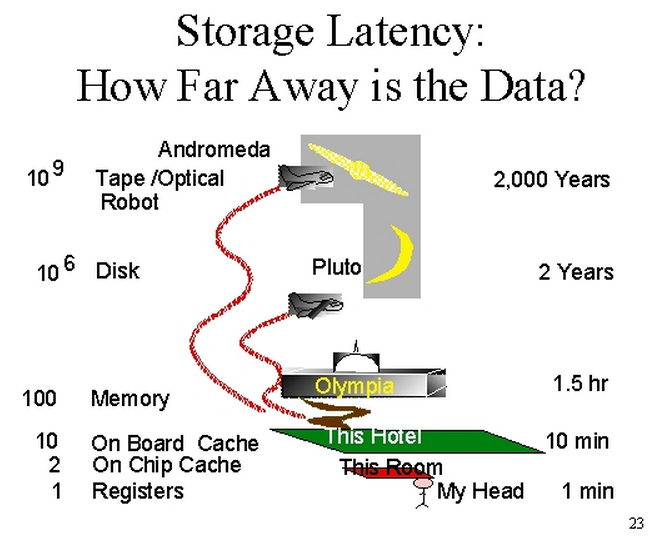
\includegraphics[width=0.67\linewidth]{storage-latency-how-far-away-is-the-data.png}}
%% \only<2>{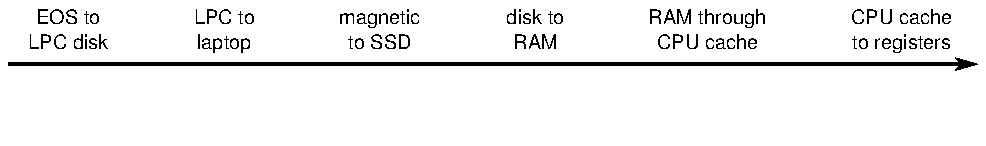
\includegraphics[width=\linewidth]{what-you-do-1.pdf}}
%% \only<3>{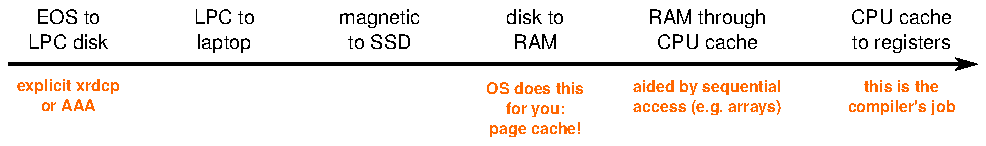
\includegraphics[width=\linewidth]{what-you-do-2.pdf}}
%% \end{center}
%% \end{frame}

%% \begin{frame}{Managing complexity}
%% \vspace{0.5 cm}
%% \begin{itemize}\setlength{\itemsep}{0.4 cm}
%% \item Python is one of the slowest languages available, and yet I used it for the high-speed mass calculation.
%% \item<2-> Actually, I just set up the calculation in Python and let it run in compiled code (Numpy). Python makes you think in terms of ``slow control'' and ``fast math.''
%% \item<3-> The slow, dynamic, abstract programming model has value: it reaches out to match the way we (humans) think.
%% \item<4-> But once we've specified a mathematical task, we want it to get out of the way.
%% \end{itemize}
%% \end{frame}

%% \begin{frame}{Getting the data at full speed}
%% \vspace{0.5 cm}
%% ROOT data are stored in an efficient format--- arrays like the ones in the high-speed mass calculation. (TBranches chopped up into TBaskets\ldots)

%% \vspace{1 cm}
%% \uncover<2->{\textcolor{darkblue}{But {\tt TTree::GetEntry} is slow:} pieces of each array are spliced into local variables each time it's called. (Also, it thwarts vectorization, has virtual function calls\ldots)}

%% \vspace{1 cm}
%% \uncover<3->{Accessing the data without {\tt GetEntry} is an order of magnitude faster.

%% \vspace{0.2 cm}
%% We're adding a method to ROOT \only<3>{6.12 (next version)}\only<4>{\xcancel{6.12 (next version)} 6.14 (next summer)} to dump data directly into Numpy arrays.}
%% \end{frame}

%% \begin{frame}{Illustration using NanoAOD decompression rate studies}
%% \begin{center}
%% \textcolor{darkblue}{\large Hint: vertical scale on right is 30$\times$ higher, reaches 0.5~MHz}
%% \end{center}

%% \begin{columns}
%% \column{0.45\linewidth}
%% \mbox{ } \hfill Reading through {\tt GetEntry} \hfill \mbox{ }

%% 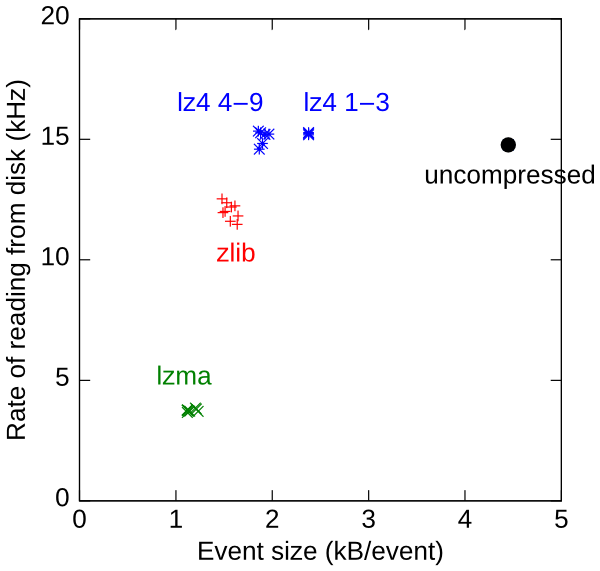
\includegraphics[width=\linewidth]{read.png}

%% \column{0.45\linewidth}
%% \mbox{ } \hfill New ROOT-to-Numpy method \hfill \mbox{ }

%% 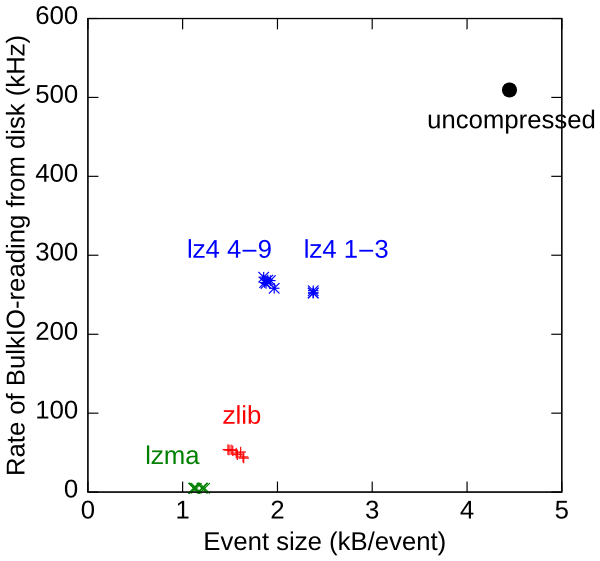
\includegraphics[width=\linewidth]{bulk.png}

%% \end{columns}
%% \end{frame}

%% \begin{frame}{Next summer is a long time to wait\ldots}
%% \vspace{0.5 cm}
%% So I wrote this access method in pure Python+Numpy:

%% \begin{center}
%% \href{https://github.com/scikit-hep/uproot}{\textcolor{blue}{\Large https://github.com/scikit-hep/uproot}}
%% \end{center}

%% 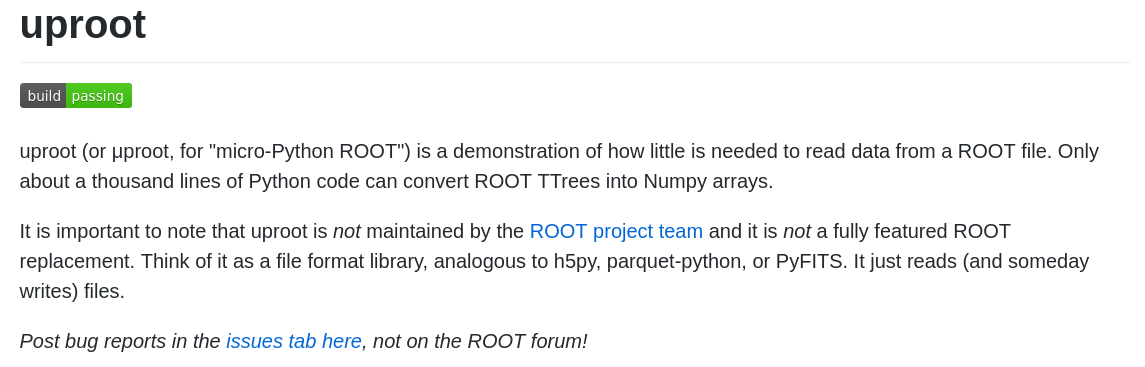
\includegraphics[width=\linewidth]{uproot.png}

%% \begin{center}
%% \Large \textcolor{red}{\tt pip install uproot --user}
%% \end{center}
%% \end{frame}

%% \begin{frame}{But\ldots\ Python is slow!}
%% \vspace{0.4 cm}
%% {\large If you're reading a reasonably large file (GB+), most of the time is spent in a Numpy call, not Python.}

%% \vspace{0.3 cm}
%% \begin{uncoverenv}<2->
%% \begin{tabular}{l c c c}
%% & \underline{Time to open file}$^{\mbox{\scriptsize *}}$ & & \\
%% C++/{\tt GetEntry} & 0.50 sec & & \\
%% Python/uproot & 0.03 sec & & \\
%% & & & \\
%%  & \underline{Time to read file} & \underline{Event rate} & \underline{Data rate} \\
%% C++/{\tt GetEntry} & 4.62 sec & 1.9 MHz & \textcolor{white}{0}230 MB/sec \\
%% Python/uproot & 0.93 sec & 9.2 MHz & 1160 MB/sec \\
%% & & & \\
%% & \underline{Time to read 1 branch} & \underline{Event rate} & \underline{Data rate} \\
%% C++/{\tt GetEntry} & 0.256 sec & \textcolor{white}{0}33 MHz & \textcolor{white}{0}260 MB/sec \\
%% Python/uproot & 0.064 sec & 133 MHz & 1020 MB/sec
%% \end{tabular}

%% \vspace{0.5 cm}
%% {\scriptsize $^{\mbox{\scriptsize *}}$from \href{https://indico.cern.ch/event/567550/contributions/2628878/}{\textcolor{blue}{Jakob Blomer's 2017 ACAT talk}} about ROOT performance, 1 GB uncompressed, flat table from LHCb.}
%% \end{uncoverenv}

%% \vspace{-6.6 cm}\hfill\begin{minipage}{0.3\linewidth}
%% \begin{uncoverenv}<3->
%% \begin{center}
%% \large
%% \textcolor{darkblue}{about 5$\times$ faster than C++/{\tt GetEntry}}

%% \vspace{0.1 cm}
%% \textcolor{darkblue}{(new method in ROOT 6.14 is 30$\times$)}
%% \end{center}
%% \end{uncoverenv}
%% \vspace{6.6 cm}
%% \end{minipage}
%% \end{frame}

%% \begin{frame}{But\ldots\ Python's GIL prevents parallelization, right?}
%% \vspace{0.4 cm}
%% {\large Python's Global Interpreter Lock (GIL) slows down parallelization of {\it Python statements,} but not external calls that release this lock.}

%% \vspace{0.35 cm}
%% \textcolor{darkblue}{uproot scales up to about 30 threads \mbox{(Knight's Landing with 128 threads shown below).\hspace{-1 cm}}}

%% \vspace{0.35 cm}
%% \begin{columns}
%% \column{0.4\linewidth}
%% \mbox{ } \hfill scaling of whole-file reading \hfill \mbox{ }

%% \vspace{0.2 cm}
%% 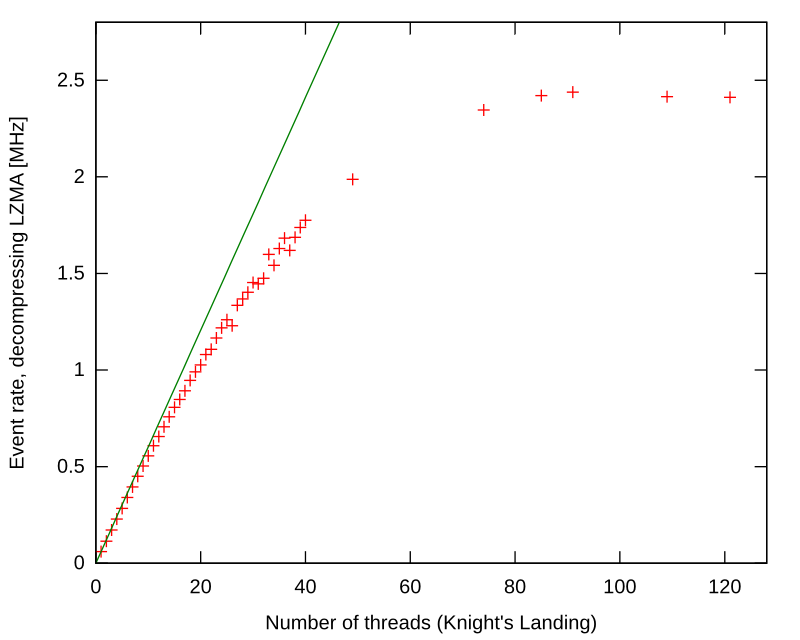
\includegraphics[width=\linewidth]{uproot-scaling.png}

%% \column{0.4\linewidth}
%% \mbox{ } \hfill scaling of single-branch reading \hfill \mbox{ }

%% \vspace{0.2 cm}
%% 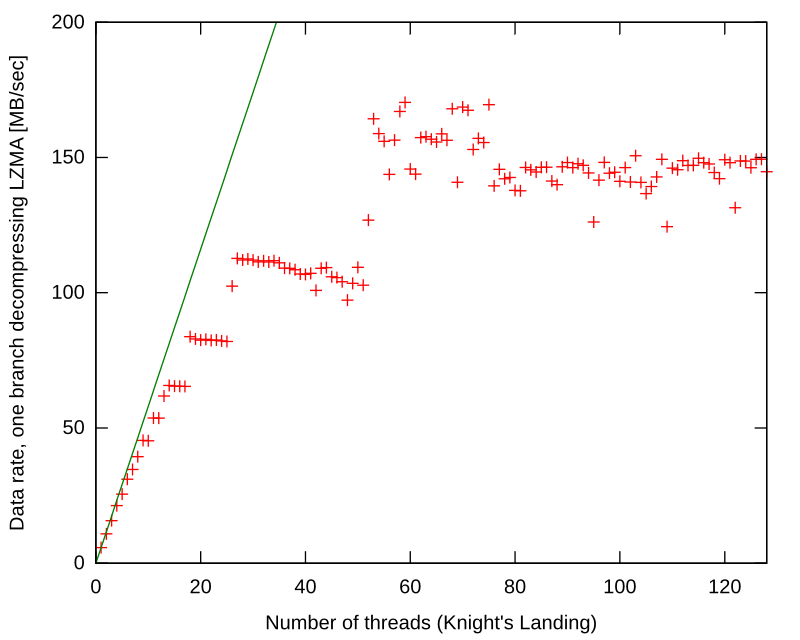
\includegraphics[width=\linewidth]{uproot-scaling-2.png}
%% \end{columns}
%% \end{frame}

%% \begin{frame}{}
%% \begin{center}
%% \LARGE So let's try it out!
%% \end{center}
%% \end{frame}

%% \begin{frame}{Nested data structures}
%% \vspace{0.5 cm}
%% {\large The crux of the problem is that our objects contain {\it variable-length} structures.}

%% \vspace{0.25 cm}
%% \begin{columns}
%% \column{0.5\linewidth}
%% 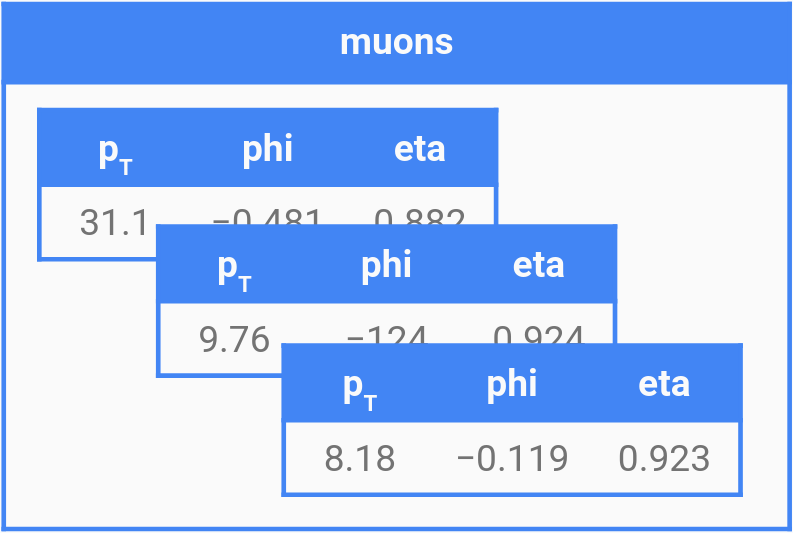
\includegraphics[width=\linewidth]{muons-as-objects.png}

%% \column{0.5\linewidth}
%% 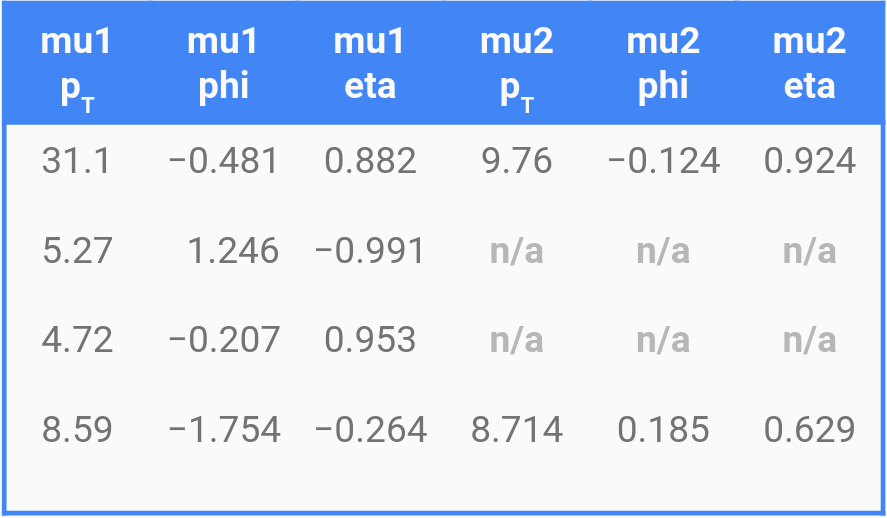
\includegraphics[width=\linewidth]{muons-as-a-table.png}
%% \end{columns}

%% \vspace{0.25 cm}
%% \uncover<2->{Most of the Big Data tools don't deal with nested structures in a first-class (optimized) way, but \href{https://youtu.be/jvt4v2LTGK0}{\textcolor{blue}{I've been trying to raise interest}} in this problem and there are a few instances where it's come up in industry, such as \href{https://issues.apache.org/jira/browse/SPARK-22231}{\textcolor{blue}{Netflix's proposed additions to Spark}}.}
%% \end{frame}

%% \begin{frame}[fragile]{Nested data structures}
%% \vspace{0.5 cm}
%% The problem of {\it storing} these data as efficient columnar arrays is solved (by ROOT in the 1990s and then Google in 2010).

%% \vspace{0.2 cm}
%% \begin{uncoverenv}<2->
%% Given data like {\tt\small \textcolor{white}{[}\textcolor{blue}{[}\textcolor{violet}{[}\textcolor{darkorange}{a}, \textcolor{darkorange}{b}, \textcolor{darkorange}{c}, \textcolor{darkorange}{d}\textcolor{violet}{]}, \textcolor{violet}{[]}, \textcolor{violet}{[}\textcolor{darkorange}{e}, \textcolor{darkorange}{f}\textcolor{violet}{]}\textcolor{blue}{]}, \textcolor{blue}{[]}, \textcolor{blue}{[}\textcolor{violet}{[}\textcolor{darkorange}{g}\textcolor{violet}{]}\textcolor{blue}{]}\ \textcolor{white}{]}}, \mbox{we can store it as\hspace{-1 cm}}
%% \end{uncoverenv}

%% \begin{uncoverenv}<3->
%% \textcolor{white}{Given data like}
%%              {\tt\small \textcolor{blue}{[0,\ \ \ \ \ \ \ \ \ \ \ \ \ \ \ \ \ \ \ \ \ \ \ \ \ \ 3,\ \ 3,\ \ \ 4]}} \textcolor{gray}{(outer list offsets)}

%% \textcolor{white}{Given data like}
%%              {\tt\small \textcolor{violet}{[\ 0,\ \ \ \ \ \ \ \ \ \ \ \ 4,\ \ 4,\ \ \ \ \ \ \ \ \ \ \ \ 6,\ \ 7]}} \textcolor{gray}{(inner list offsets)}

%% \textcolor{white}{Given data like}
%%              {\tt\small \textcolor{darkorange}{[\ \ a,\ b,\ c,\ d,\ \ \ \ \ \ \ e,\ f,\ \ \ \ \ \ \ \ \ g\ \ \ ]}} \textcolor{gray}{(attribute data)}
%% \end{uncoverenv}

%% \vspace{0.2 cm}
%% \uncover<4->{This representation is Apache Arrow; ROOT only splits one level deep.}

%% \vspace{0.2 cm}
%% \uncover<5->{What's missing is the ability to efficiently run algorithms over it.}

%% \vspace{0.2 cm}
%% \begin{columns}[t]
%% \column{0.325\linewidth}
%% \begin{uncoverenv}<6->
%% \mbox{\hspace{-0.1 cm}\underline{we want to write}}

%% \vspace{-0.25 cm}
%% \small
%% \begin{minted}{python}
%% for outer in lists:
%%    for inner in outer:
%%       for char in inner:
%%          print(char)
%% \end{minted}
%% \end{uncoverenv}

%% \column{0.65\linewidth}
%% \begin{uncoverenv}<7->
%% \mbox{\hspace{-0.1 cm}\only<7>{most software (like ROOT's {\tt GetEntry}) turns the arrays\hspace{-1 cm}}\only<8>{\underline{ideally, we'd change the code to fit the data}}\only<9->{\underline{or even (special case of exhaustive nested loops)}}}

%% \only<7>{back into lists and sublists}

%% \small
%% \vspace{-0.25 cm}
%% \begin{onlyenv}<8>
%% \begin{minted}{c}
%% for (i = 0; i < 3; i++)
%%    for (j = outer[i]; j < outer[i+1]; j++)
%%       for (k = inner[j]; k < inner[j+1]; k++)
%%          print(data[k]);
%% \end{minted}
%% \end{onlyenv}
%% \begin{onlyenv}<9->
%% \begin{minted}{c}
%% for (k = 0; k < inner[outer[3]]; k++)
%%    print(data[k]);
%% \end{minted}
%% \end{onlyenv}
%% \end{uncoverenv}
%% \end{columns}
%% \end{frame}

\begin{frame}{Next software product: code transformation/compilation}
\vspace{0.3 cm}
Actually, it's a research project\footnote{IEEE Big Data, \href{https://arxiv.org/abs/1708.08319}{\textcolor{blue}{arXiv:1708.08319}} [cs.PL]}; the code is not as polished as uproot.

\vspace{0.25 cm}
\uncover<2->{\textcolor{darkblue}{Workflow:} uproot converts ROOT on-the-fly to Apache Arrow and your analysis code gets converted to run on the Arrow data (compiled).}

\vspace{-0.5 cm}
\begin{columns}[t]
\column{0.5\linewidth}
\begin{center}
\uncover<3->{\underline{Why Arrow?}}

\vspace{0.25 cm}
\uncover<4->{\small Nested, columnar data representation shared among many Big Data projects.}

\uncover<4->{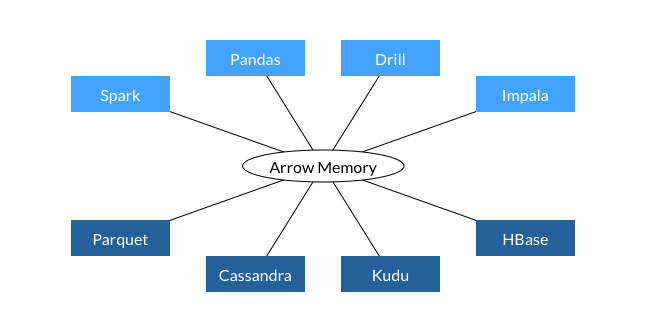
\includegraphics[width=\linewidth]{apache-arrow.png}}
\end{center}

\column{0.5\linewidth}
\begin{center}
\uncover<5->{What do you call a function that}

\uncover<5->{\underline{has been transformed to run on Arrow?}}

\vspace{0.2 cm}
\uncover<6->{
\includegraphics[width=0.8\linewidth]{Arrowed_Full.png}}

\vspace{-0.2 cm}
\end{center}
\end{columns}
\end{frame}

\begin{frame}{}
\vspace{0.75 cm}
\begin{center}
\mbox{\hspace{-1 cm}\begin{columns}
\column{1.2\linewidth}
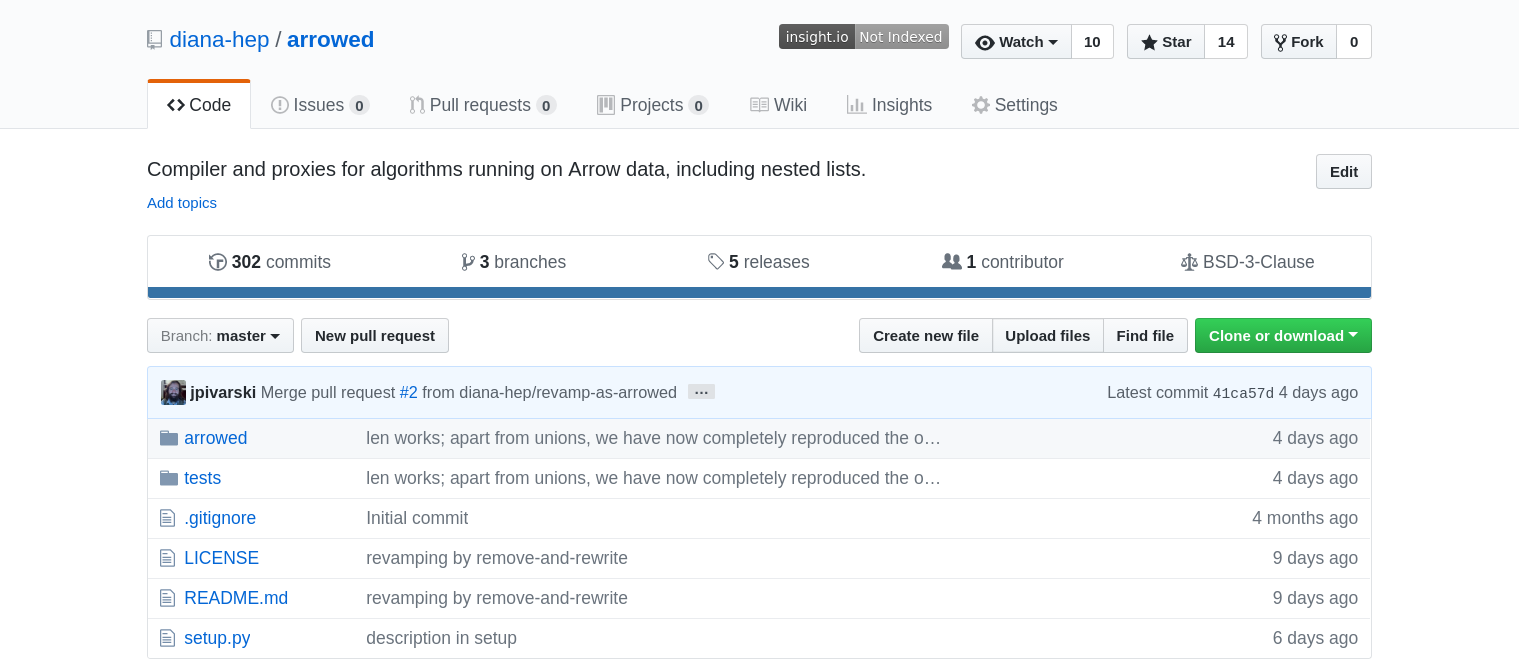
\includegraphics[width=\linewidth]{arrowed.png}
\end{columns}}
\end{center}
\end{frame}


\end{document}
